The effect of free-precession and the inclusion of an EM torque was
considered analytically by \citet{Jones2001}. They calculated several useful
results for the magnitude of variations in the residual; we can use these to
verify our simulations. By simulating the residuals directly, we can improve
on their results by understanding some of the more subtle features.

\subsection{Understanding the wobble angle}
The analytic calculations of \citet{Jones2001} are based on the wobble angle 
$\wobbleangle$ which the spin-vector makes with the axis about which it precesses.
This axis depends on the mass distribution, and any applied torques. Before
continuing we discuss what this wobble angle is given by in different cases.

To understand the wobble angle we refer to figure \ref{fig: reference plane}
illustrating the so-called reference plane from \citet{Jones2001}
\begin{figure}
    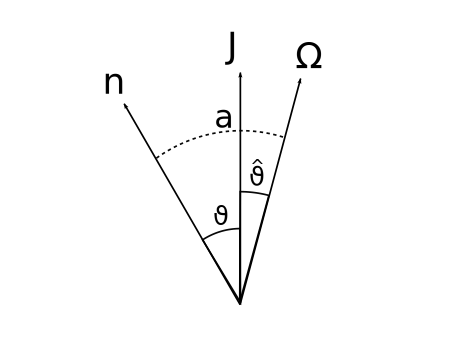
\includegraphics[width=0.2\textwidth]{/home/greg/Neutron_star_modelling/Illustrations/ReferencePlane/ReferencePlane.pdf}
    \caption{The reference plane containing the angular momentum vector $\spin$,
    the angular momentum vector $\L$ and the symmetry axis $n$ lying along the
    body-frame $\z$ axis. The dotted line indicates the polar angle $a$ between
    the body-frame $\z$ axis and the spin vector.}
    \label{fig: reference plane}
\end{figure}
This reference plane is a direct result of the relation 
\begin{align}
    L_{a} = I_{ab} \omega_{b} &&& I_{ab} = I_{0} \delta_{ab} + \epsI\delta_{3a}\delta_{3b}
\end{align}
since $\mathbf{n}$ lies along the $\z$ axis of the body frame. It was shown by
\citet{Jones2001} that for nearly spherical bodies
\begin{equation}
    \hat{\theta} \approx \epsI \sin\theta \cos\theta.
\end{equation}
Taking also the limit that $\theta \ll 1$ it can be shown that
\begin{equation}
    \hat{\theta} \approx \epsI \theta
\end{equation}
and so when comparing the two angles $\hat{\theta} \ll \theta$ such that 
$a\approx \theta$.

For a biaxial body free of torques, the spin vector precesses about the
symmetry axis of the moment of inertia $\mathbf{n}$. Using the approximations
mentioned above then the wobble angle is given by
\begin{equation}
    \wobbleangle \approx \theta.
\end{equation}
Therefore, solutions without precession correspond to $a=0$.
%For triaxial bodies it can precess
%about either of the stable axis of the moment of inertia \citep{Landau1969}. 

Including the EM torque from equation \eqref{eqn: torque} introduces two effects:
the first and the largest is the transformation induced by the anomalous torque
which causes the spin-vector to precess about the principle axis of an
\emph{effective} body-frame. This has already been discussed in chapter \ref{sec:
effective body frame} and results in a wobble angle
\begin{equation}
    \wobbleangle \approx \theta - \beta
    \label{eqn: wobble angle no SD}
\end{equation}
where $\beta$ is the rotation from the body-frame to the effective body-frame.
In this case non-precessing solutions correspond to $a \approx \beta$.

The second, smaller effect is that, even without the anomalous torque the spin-down 
torque introduces a time-varying component to the angular momentum vector. Which
will change the axis of precession. The magnitude of this time
varying component is given by 
\begin{equation}
|\dot{\L}| \sim L \omega \hat{\theta}
\end{equation} 
this can be equated to the magnitude of the spindown torque
\begin{equation}
|T_{\mathrm{sd}}| = I_{0}|\dot{\spin}|
\end{equation}
rearranging for the angle between the spin-vector and angular momentum yeilds
\begin{equation}
    \hat{\theta} = \frac{I_{0}\dot{\omega}}{I \omega^{2}} = \frac{P}{\tauS}
\end{equation}
The wobble angle due to this spin-down torque is then given by 
\begin{align}
    \wobbleangle_{\mathrm{SD}} & = \theta + \hat{\theta}\\
                 & = \hat{\theta}\left(1 + \frac{1}{\epsI}\right) \\
                 & = \frac{P}{\tauS}\left(1 + \frac{1}{\epsI}\right) \\
                 & \approx \frac{P}{\tauS}{\frac{1}{\epsI}}
    \label{eqn: spindown wobble angle}
\end{align}
Therefore we can write the wobble angle in general as
\begin{equation}
    \wobbleangle = \theta - \beta + \frac{P}{\tauS}\frac{1}{\epsI}
    \label{eqn: wobble angle}
\end{equation}
Now for solutions where the precession is important the final term
will be negligable and so we generally refer to equation \eqref{eqn: wobble angle no SD}.
However, when we set up initial conditions to minimise the precession: either
$a_{0}=0$ for free precession or $a_{0} = \beta$ when incuding the anomalous
torque; the approximations we made earlier become important. Now the wobble angle
due to the spindown can dominate and so we should use the full expression in
equation \eqref{eqn: wobble angle}.


\subsubsection{Effect of free precession on the phase residual: geometric effect}
\citet{Jones2001} analysed the geometric effect that precession will have on
the timing residual. This was done by considering the motion of the magnetic
dipole in the inertial frame as the superposition of motions due to the fast
rotation period and the slow precession. The results
must be separated into two cases when $\theta > \chi$ and $\theta < \chi$. Of
these two the authors argue that `the wobble angle  of rapidly rotating
stars are limited to small values by the finite crustal breaking strain'. Therefore, 
the second case $\theta < \chi$ holds greater physical relevance and so we 
focus on this region of parameter space. The phase residual for such NSs was 
shown to be given by  
\begin{equation}
    \Delta\Phi^{49}(t) = -\wobbleangle \cot\chi\cos(\dot{\psi t}),
    \label{eqn: Jones 49}
\end{equation}
where the superscript here refers to the equation number from \citet{Jones2001}.
For a freely precession star $\dot{\psi}=\epsI \f$ is the constant free
precession frequency. Therefore, the magnitude of variations is given by 
$|\Delta\Phi^{49}|=\wobbleangle \cot(\chi)$. 

Equation \eqref{eqn: Jones 49} is calculated in the absence of any EM torque.
Nevertheless, it is still appropriate when such a torque is applied provided
that the geometric effect is stronger that any other (these are discussed in
the next few sections). As such we begin by simulating a NS with the properties
listed in table \ref{tab: 49 verification properties}. Nonphysical values of the
rotation frequency and magnetic field have been used to aid the computational
speed. The resulting phase residual, in cycles, is given in figure \ref{fig:
PR 49}.

%\begin{table}[ht]
    %\centering
    %\input{49_verification.tex}
    %\caption{}
    %\label{tab: 49 verification properties}
%\end{table}

%\begin{figure}[ht]
%\centering
	%\includegraphics[width=0.7\textwidth]{49_verification.pdf}
%\caption{The phase residual in cycles for a simulated NS with the properties described in table \ref{tab: 49
%verification properties}. This is used to illustrate the agreement with the magnitude
%of variations from equation \eqref{eqn: Jones 49} taken from \citet{Jones2001}.}
%\label{fig: TR 49}
%\end{figure}

\begin{figure}[htb]
\begin{floatrow}
\ffigbox{%
\includegraphics[width=0.5\textwidth]{49_verification.pdf}
}{%
  \caption{The phase residual in cycles for a simulated NS with the properties described in table \ref{tab: 49
verification properties}. This is used to illustrate the agreement with the magnitude
of variations from equation \eqref{eqn: Jones 49} taken from \citet{Jones2001}.}%
  \label{fig: PR 49}
}
\capbtabbox{%
  \input{\TimingResidualsDir/49_verification.tex}
}{%
  \caption{}%
  \label{tab: 49 verification properties}
}
\end{floatrow}
\end{figure}

\FloatBarrier
\subsubsection{Effect of free precession on the phase residual: effect of the 
            electromagnetic torque}
Considering a vacuum point-dipole spin-down torque (like the one introduced in 
\ref{sec: defining the model}) \citet{Jones2001} found that the EM torque can
amplify the geometric effect of equation \eqref{eqn: Jones 49}. The magnitude
of variation due to EM torque is given by 
\begin{equation}
    |\Delta\Phi^{63}| = \frac{1}{\pi}\left(\frac{\tau_{P}}{P}\right)
    \left(\frac{\tau_{P}}{\tau_{S}}\right) 
                                    |\Delta\Phi^{49}|
\label{eqn: Jones 63}
\end{equation}
The two ratios of time-scales define an `amplification factor'; this increases
the magnitude of phase residuals for young pulsars with short periods.

We simulate such a star using the properties in table \ref{tab: 63 verification
properties} noting that the amplification factor is $\sim 3$ when including the
factor of $\pi$. The resulting phase residual is plotted in figure \ref{fig: PR
63} along with the magnitude of variations due to free precession along and the
amplification due to the EM torque. The magnitude of the simulated
phase-residuals are found to agree well with the analytic results of equation
\eqref{eqn: Jones 63}.

%\begin{table}[ht]
%    \centering
%     \begin{tabular}{ccl}
\multicolumn{3}{c}{Simulation parameters} \\
\hline
$\omega_0$  &=& 1550.0 rad/s\\
$B_0$  &=& $ 1.581\times 10^{14} $ G \\
$\chi$  &=& 70.00$^{\circ}$ \\
$a_0$ &=& 2.00$^{\circ}$ \\
$\tilde{\theta}$ &= & 2.01$^{\circ}$
\end{tabular}
    
%    \caption{}
%    \label{tab: 63 verification properties}
%\end{table}
%
%\begin{figure}[ht]
%\centering
%	\includegraphics[width=0.7\textwidth]{63_verification.pdf}
%\caption{The phase residual in cycles for a simulated NS with the properties described in table \ref{tab: 49
%verification properties}. This is used to illustrate the agreement with the magnitude
%of variations from equation \eqref{eqn: Jones 49} taken from \citet{Jones2001}.}
%\label{fig: TR 63}
%\end{figure}

\begin{figure}[htb]
\begin{floatrow}
\ffigbox{%
\includegraphics[width=0.5\textwidth]{63_verification.pdf}
}{%
  \caption{The phase residual in cycles for a simulated NS with the properties described in table \ref{tab: 63
verification properties}. This is used to illustrate the agreement with the magnitude
of variations from equation \eqref{eqn: Jones 63} taken from \citet{Jones2001}.}%
  \label{fig: PR 63}
}
\capbtabbox{%
   \begin{tabular}{ccl}
\multicolumn{3}{c}{Simulation parameters} \\
\hline
$\omega_0$  &=& 1550.0 rad/s\\
$B_0$  &=& $ 1.581\times 10^{14} $ G \\
$\chi$  &=& 70.00$^{\circ}$ \\
$a_0$ &=& 2.00$^{\circ}$ \\
$\tilde{\theta}$ &= & 2.01$^{\circ}$
\end{tabular}
    
}{%
  \caption{}%
  \label{tab: 63 verification properties}
}
\end{floatrow}
\end{figure}

%In figure \ref{fig: TR no torque} we plot the timing residuals as calculated in
%the torque free model for three values of $\chi$. It is worth noting that the
%power law spin down assumes that the star is in fact spinning down; without the
%torque this model can't not spin down. We can however interpret these results
%as the effect of precession on timing residuals in the limit for which the
%variation due to precession is much stronger than the spin down.
%%\begin{figure}[ht]
%%\centering
%%	\includegraphics[width=0.7\textwidth]{Timing_residuals_no_torque.pdf}
%%\caption{Plot of the timing residuals for three angles of $\chi$ in the torque
%%         free model showing different types of behaviour. }
%%\label{fig: TR no torque}
%%\end{figure}
%The results show that the precession induces a periodic variation on the
%precession timescale, the magnitude is proportional to the angle $\chi$. We 
%also find the results are dependant on the initial angle $a_{0}$.

\subsubsection{Effect of free precession on phase residuals: orthogonal rotator}

In analysing observations of free precession \citet{Jones2001} applied the
model to PSR B1821-11: a pulsar with a strongly periodic residual that has been
cited as a strong candidate for free precession \citet{Stairs2000}. From the
variations in pulse shape an estimate can be made of the wobble angle
$\wobbleangle \sim 3^{\circ}$. Finding that the amplification factor was
important for this pulsar (it can be calculated to be $\approx 380$), 
\citet{Jones2001} attempted to extract the wobble
angle by inverting \eqref{eqn: Jones 65}. This yields a wobble angle that
disagreed with the estimation from a pulse shape variations. The author
concluded that the strong harmonic periodicity's suggested the dipole was
nearly orthogonal e.g. $\chi \approx \pi/2$.  This required expansions of the
phase modulation resulting in an estimate
\begin{equation}
    |\Delta\Phi^{75}| = \frac{1}{4\pi} \frac{\tau_{P}^{2}}{\tau_{S} P} \theta^{2}
    \label{eqn: Jones 75}
\end{equation}

In figure \ref{fig: PR 75} we simulate the B1828-11 pulsar taking the values
from \citet{Stairs2000} and modifying them to allow the simulation to complete
in a reasonable time. The modification was setup such that the amplification
factor remained the same along with the ratio of timescales. The properties
of the simulation are given in \ref{tab: 75 verification properties}

\begin{figure}[htb]
\begin{floatrow}
\ffigbox{%
\includegraphics[width=0.5\textwidth]{75_verification.pdf}
}{%
  \caption{The phase residual in cycles for a simulated NS with the properties described in table \ref{tab: 75
verification properties}. This is used to illustrate the agreement with the magnitude
of variations from equation \eqref{eqn: Jones 75} taken from \citet{Jones2001}.}%
  \label{fig: PR 75}
}
\capbtabbox{%
  \input{\TimingResidualsDir/75_verification.tex}
}{%
  \caption{}%
  \label{tab: 75 verification properties}
}
\end{floatrow}
\end{figure}



